\documentclass{article}
\usepackage{iclr2026_conference,times}
\usepackage{graphicx}
\usepackage{booktabs}
\usepackage{amsmath,amssymb,amsthm}
\usepackage{url}
\usepackage{enumitem}
\usepackage{microtype}

\title{Contact State Compression Limits}

\author{Anonymous Authors\\
Paper under double-blind review}

\newtheorem{theorem}{Theorem}
\newtheorem{definition}{Definition}
\newtheorem{corollary}{Corollary}

\begin{document}
\maketitle

\begin{abstract}
Robots often compress contact state before planning or feedback control: a world model may keep only ``in contact'', a tactile encoder may keep a semantic label, or a planner may bin many contact geometries into one mode. This paper studies when that compression is not merely lossy but control-destroying. We show that if a compressed contact state aliases modes whose task-feasible action sets have empty intersection, no deterministic controller that observes only the compressed state can guarantee the local task for all aliased modes. The result suggests a repair: compress contact by control-cone signatures, splitting only those aliases that change the feasible action cone. A runnable friction-cone experiment shows the mechanism directly. Contact-count compression succeeds on 72.0% of raw-controllable local tasks and has an empty-intersection rate of 100.0%; the proposed cone-signature repair uses 6 bits over 52 groups and recovers 99.9% success, close to raw mode identity at 100.0%. The contribution is a small but sharp representational test for contact-rich robot world models: prediction-faithful compression is not enough when contact changes which actions are possible.
\end{abstract}

\section{Introduction}
Contact is where compact robot state representations become dangerous. In free space, merging nearby states often causes a graceful degradation in prediction or cost. In contact-rich manipulation and locomotion, a small hidden change in contact normal, friction cone, or sticking/sliding mode can flip the set of feasible actions. The robot does not merely predict the wrong next state; it may have no single safe action that works for all true states hidden behind the same compressed observation.

The seed problem is common in embodied intelligence. Learned world models, tactile encoders, and task-and-motion abstractions frequently replace detailed contact variables by a smaller latent or symbolic state. That move is attractive because exact contact state is high dimensional and brittle. The risk is that the compression criterion is usually predictive or semantic, while the controller needs action feasibility.

This paper asks a local question: when does compressed contact state destroy controllability? The answer is expressed through feasible-action intersections. For a task direction $g$, let $A_g(c)$ be the actions that both maintain the relevant contact constraints and make task progress in true contact mode $c$. If a representation $\phi$ merges modes $c_1$ and $c_2$ but $A_g(c_1)\cap A_g(c_2)=\emptyset$, then any policy that sees only $\phi(c_1)=\phi(c_2)$ must choose the same action for both and must fail at least one. This is a representation-level obstruction, not an optimizer weakness.

We make three contributions. First, we formalize a contact-compression failure certificate based on empty intersections of task-feasible action sets. Second, we propose contact-cone separating compression (CCSC), a repair that refines aliases by action-cone signatures rather than reconstructing full contact geometry. Third, we provide a reproducible local friction-cone experiment and a 1000-paper literature map that delimit the novelty boundary.

\section{Related Work}
Planar pushing and contact mechanics established that contact geometry and friction determine controllability \citep{mason1986,lynch1996,zhou2018,fazeli2017}. Rigid-body contact simulation and complementarity formulations made contact constraints explicit state variables for dynamics and optimization \citep{stewart1996,anitescu1997,todorov2012}. Contact-implicit and contact-invariant optimization can discover rich behaviors when the optimization problem retains enough variables to express the contact constraints \citep{mordatch2012,posa2014,toussaint2015}. Tactile and contact-state estimation work estimates hidden object or contact variables during manipulation \citep{koval2015}.

Those lines make the present result more modest and more specific. We do not claim that contact modes, friction cones, or pushing controllability are new. The gap is the compression criterion. Generic abstraction theory, including MDP model minimization \citep{givan2003}, asks when states can be merged without changing decision behavior. This paper instantiates that idea for contact dynamics with a physically interpretable certificate: merged contact modes must share task-feasible actions. The hostile prior-work set in the repository records 100 papers most likely to erode the contribution.

\section{Problem Setup}
Let $C$ be a finite set of local contact modes, $A$ a compact action set, and $G$ a family of local task directions or guards. For each $c\in C$ and $g\in G$, define a binary success predicate
\[
S(c,g,a)=1
\]
when action $a$ maintains the contact constraints required by mode $c$ and produces enough progress for task $g$. The corresponding feasible action set is
\[
A_g(c)=\{a\in A: S(c,g,a)=1\}.
\]
A contact-state compression is a map $\phi:C\rightarrow Z$. A compressed feedback policy is any $\pi:Z\times G\rightarrow A$. This covers a controller whose world model or encoder exposes $z=\phi(c)$ but not the true mode.

\begin{definition}[Control-faithful alias class]
An alias class $B_z=\{c\in C:\phi(c)=z\}$ is control-faithful for task $g$ if
\[
\bigcap_{c\in B_z: A_g(c)\neq\emptyset} A_g(c) \neq \emptyset.
\]
It is control-destroying if at least two modes in $B_z$ are individually feasible for $g$ but the intersection is empty.
\end{definition}

\section{Compression Limit}
\begin{theorem}[Empty-intersection obstruction]
Fix a task $g$ and compression $\phi$. Suppose there is an alias class $B_z$ containing modes $c_1,\ldots,c_k$ such that $A_g(c_i)\neq\emptyset$ for every $i$ but $\cap_i A_g(c_i)=\emptyset$. Then no deterministic compressed policy $\pi(z,g)$ can satisfy $S(c_i,g,\pi(z,g))=1$ for all $i$.
\end{theorem}
\begin{proof}
Because the modes share the same compressed state, the policy must choose one action $a^\star=\pi(z,g)$ for all of them. If it succeeded for every aliased mode, then $a^\star\in A_g(c_i)$ for every $i$, so $a^\star$ would lie in $\cap_i A_g(c_i)$. This contradicts the empty-intersection assumption.
\end{proof}

The theorem is local and intentionally severe. It does not say history, probing, belief-space planning, or randomized policies are useless. It says that when the first safety-critical action must already work, missing action-cone information cannot be recovered downstream.

\begin{corollary}[Prediction is insufficient]
If two contact modes are merged by a representation because they have similar predicted observations or next states under an average action distribution, but their task-feasible action sets are disjoint for a required task, prediction-faithful compression is not control-faithful for that task.
\end{corollary}

\section{Repair: Contact-Cone Separating Compression}
CCSC changes the object being compressed. Instead of preserving every contact coordinate or a semantic label, it preserves a coarse signature of feasible actions. Given probe tasks $\bar G\subset G$ and action sectors $\bar A$, each mode receives a signature
\[
\sigma(c)=\left(\mathbf{1}_{\exists a\in \bar A_j: S(c,\bar g,a)=1}\right)_{\bar g\in \bar G, j}.
\]
The repaired compression is $\phi_{\rm ccs}(c)=\sigma(c)$, optionally starting from an existing coarse representation and splitting only aliases whose signatures differ. This is not a verifier added after a controller acts. It changes what the contact state must retain: action-separating predicates.

In practice, the signature can be computed from an analytic contact model, a differentiable simulator, or action-labeled tactile data. The present paper uses the analytic route to keep the evidence auditable.

\section{Runnable Evidence}
We instantiate a local point-contact model with 64 modes, each defined by a contact normal, friction coefficient, and transmission gain. An action is a unit push direction. It is feasible for a task if it pushes into the contact, respects a Coulomb-like tangential limit, and yields positive progress along the task direction. We compare contact count, normal bins, normal-plus-friction bins, CCSC, and raw mode identity. All numbers are regenerated by \texttt{python scripts/run\_experiments.py}.

\begin{table}[t]
\centering
\begin{tabular}{lrrrr}
\toprule
Representation & Groups & Bits & Success & Empty alias rate \\
\midrule
contact count & 1 & 0 & 0.720 & 1.000 \\
normal 4 & 4 & 2 & 0.980 & 0.105 \\
normal 8 & 8 & 3 & 0.994 & 0.039 \\
normal8 mu2 & 16 & 4 & 0.999 & 0.004 \\
cone signature repair & 52 & 6 & 0.999 & 0.007 \\
raw mode & 64 & 6 & 1.000 & 0.000 \\
\bottomrule
\end{tabular}
\caption{Compression results conditioned on tasks that are feasible with raw mode identity. Empty alias rate is the fraction of alias group/task pairs with individually feasible modes but no common action.}
\label{tab:results}
\end{table}

\begin{figure}[t]
\centering
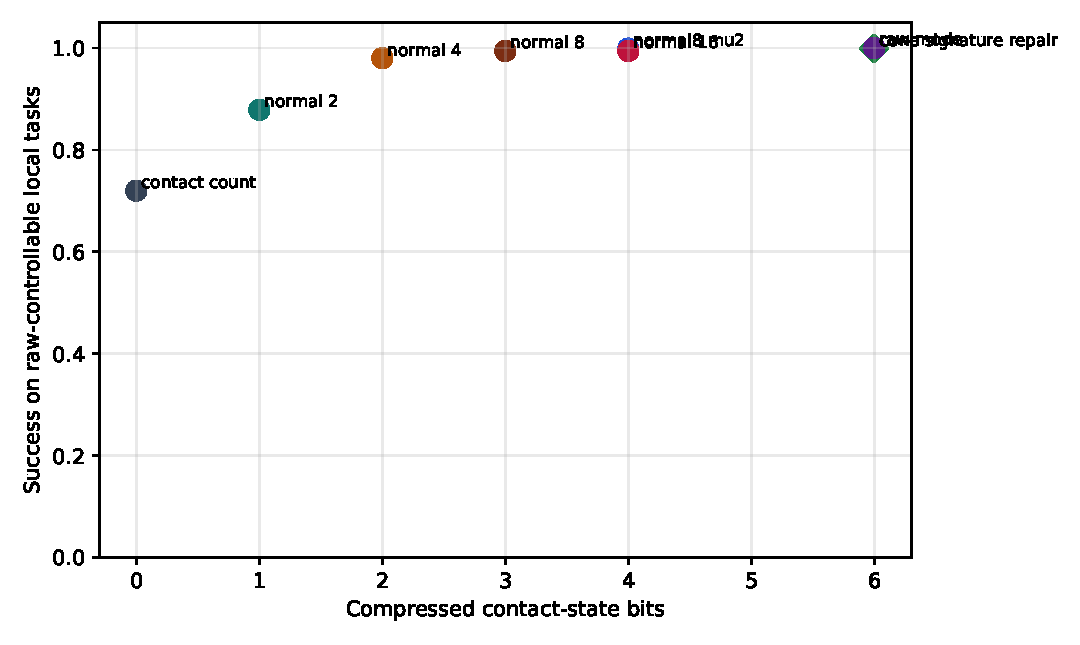
\includegraphics[width=0.76\linewidth]{../figures/success_vs_bits.pdf}
\caption{Contact-count compression throws away the distinctions that choose feasible actions. CCSC recovers most raw-mode success with fewer represented groups than exact mode identity.}
\label{fig:success}
\end{figure}

\begin{figure}[t]
\centering
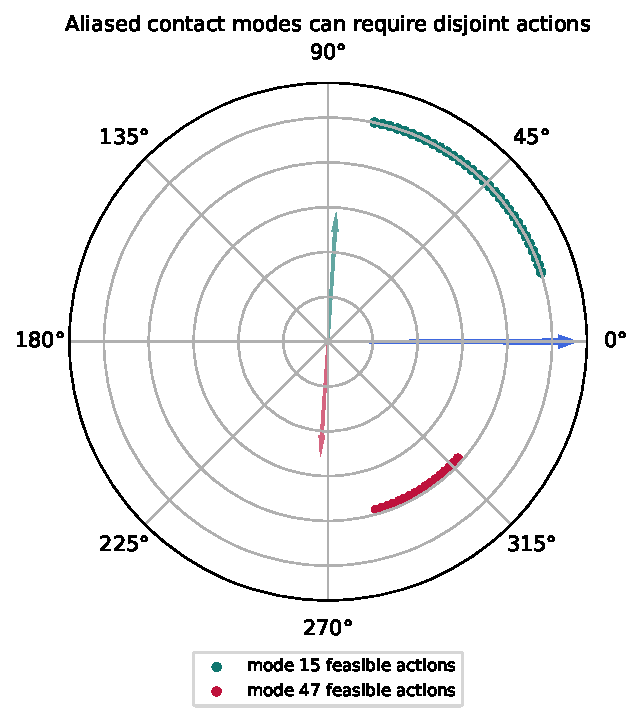
\includegraphics[width=0.48\linewidth]{../figures/contact_cones_alias.pdf}
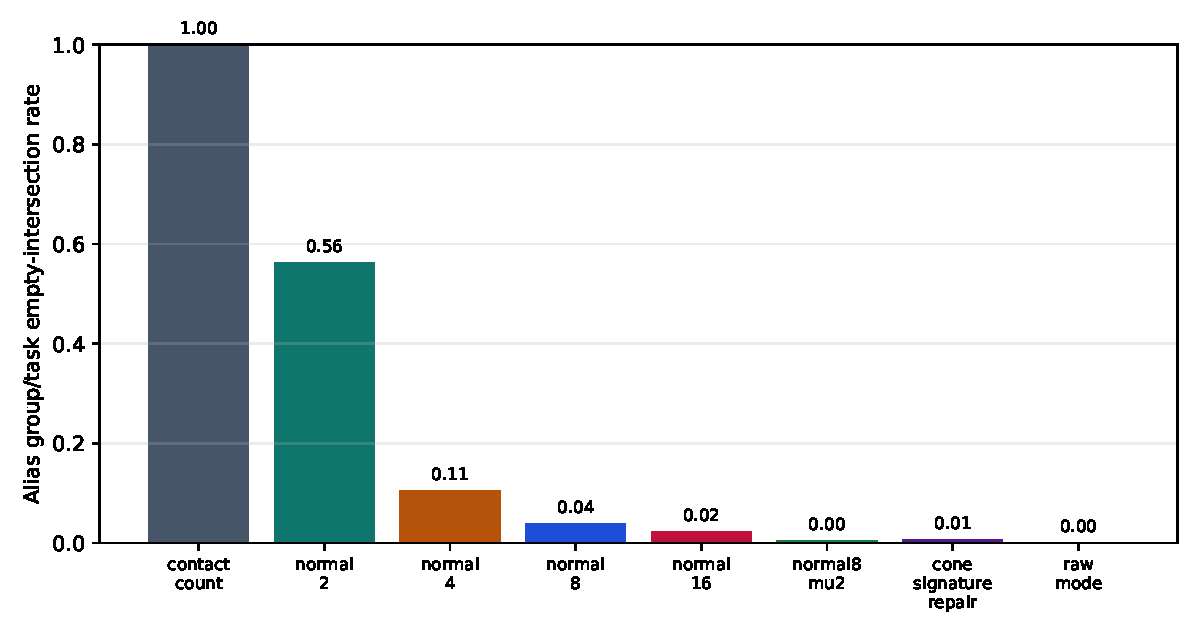
\includegraphics[width=0.48\linewidth]{../figures/empty_intersection_rate.pdf}
\caption{Left: two modes hidden behind the same contact-count state can require disjoint action sectors for the same task. Right: empty intersections fall as compression preserves contact-cone information.}
\label{fig:cones}
\end{figure}

The experiment supports the theorem's mechanism. The coarse representations do not fail because the local dynamics are hard to optimize; the policy is given the best group action by exhaustive search over action directions. They fail because the alias class itself has no common feasible action. CCSC improves success by splitting aliases along the same object that appears in the proof: feasible action signatures.

\section{Limitations}
The evidence is local and model-based. It does not prove that a particular robot foundation model currently destroys contact controllability, nor does it validate CCSC on hardware. The theorem is one-step and deterministic; if the robot can safely probe, maintain a belief, or delay the task, some aliases may become recoverable. The repair also needs a source of action-feasibility labels. These limitations are acceptable for the paper's central claim: before adding more planning machinery, a contact representation should be tested for control-faithful alias classes.

\section{Reproducibility Statement}
The repository contains the full sweep, experiment, and build scripts. The literature matrix is in \texttt{docs/related\_work\_matrix.csv}. Experiment outputs are in \texttt{results/} and figures in \texttt{figures/}. The ICLR template fetch status was \texttt{official\_template\_ready}; source details are written to \texttt{paper/template\_source.md}.

\bibliography{references}
\bibliographystyle{iclr2026_conference}

\end{document}
